\xiti
\begin{xiaotis}
\begin{enhancedline}

\xiaoti{已知棱台两底面的面积分别为 $245\;\pflm$,$80\;\pflm$,截得这个棱台的棱锥的高是 35 cm。求这个棱台的体积。}

\xiaoti{两底面边长分别是 15 m、10 m 的正三棱台,它的侧面积等于两底面面积的和。求这个三棱台的体积。}

\xiaoti{已知棱台的体积是 $76\;\lflm$,高是 6 cm,一个底面面积是 $18\;\pflm$。求这个棱台的另一个底面面积。}

\xiaoti{棱台的高为 20 cm,体积为 $1720\;\lflm$,两底面对应边的比是 $5:8$。求两底面面积。}

\xiaoti{已知过三棱台上底面的一边与一条侧棱平行的一个截面,它的两个顶点是下底面两边的中点。 求棱台被分成两部分的体积的比。}

\begin{figure}[htbp]
    \centering
    \begin{minipage}[b]{7cm}
        \centering
        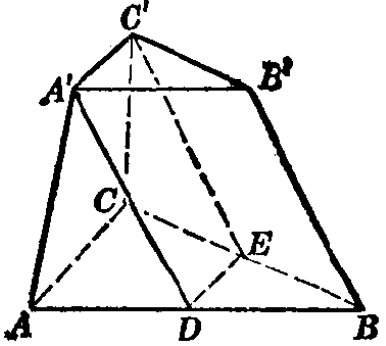
\includegraphics[width=5cm]{../pic/ltjh-ch2-xiti14-05.png}
        \caption*{(第 5 题)}
    \end{minipage}
    \qquad
    \begin{minipage}[b]{7cm}
        \centering
        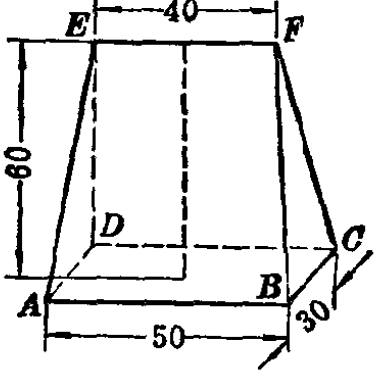
\includegraphics[width=5cm]{../pic/ltjh-ch2-xiti14-12.png}
        \caption*{(第 12 题)}
    \end{minipage}
\end{figure}


\xiaoti{圆台的高为 3,一个底面半径是另一个底面半径的 2 倍,母线与下底面所成的角为 $45^\circ$。求它的体积。}

\xiaoti{圆台的体积是 $234\sqrt{3}\, \pi \;\lflm$,侧面展开图是半圆环,它的大半径等于小半径的 3 倍。求这个圆台的上底面半径。}

\xiaoti{证明:当上、下底面半径的大小相近时,圆台的体积可近似地表示为 $V \approx \dfrac{1}{12} c^2h$,其中 $c$ 是中截面周长,$h$ 是高。}

\xiaoti{有一草垛,上部是圆锥形,下部是圆台形。圆锥高 0.7 m,底面周长是 5.1 m;
    圆台高 1.5 m,下底面周长是 4 m。 如果每立方米草重 300 斤,利用上题结果,
    估算这个草垛的重量(保留一位有效数字)。
}

\begin{withstar}

\xiaoti{有一沙堆,它的上底面和下底面是互相平行的两个矩形,各侧面都是梯形,上底面的边长约是 5.2 m 和 3.4 m,
    下底面的边长约是 7.3 m 和 4.2 m,上下底面距离约是 2.5 m。 求这堆沙有多少立方米。
}

\xiaoti{有一碴石堆,它的下底呈矩形,长宽分别是 $a$ 米和 $b$ 米,上、下底面互相平行,
    各侧面与地面成 $45^\circ$ 角,碴石堆高 $h$ 米。求它的体积。
}

\xiaoti{楔体的底面 $ABCD$ 是边长为 50 cm 和 30 cm 的矩形,棱 $EF$ 平行于 $AB$,
    与底面距离是 60 cm,长是 40 cm。求这个楔体的体积。
}

\xiaoti{长方台的上底面边长是 $a$、$b$,下底面与它们平行的边长是 $a'$、$b'$,高是 $h$。求证:长方台的体积是
    $$ V = \exdfrac{1}{6} h [2(ab + a'b') + ab' + a'b] \juhao $$
}

\end{withstar}

\end{enhancedline}
\end{xiaotis}

